\chapter{High throughput QTL mapping using correlated traits}
\thispagestyle{empty}
\label{chap:ctlmapping}

\emph{In this chapter we develop a new methodology to be used in quantitative genetics 
called Correlated Traits Locus (CTL) mapping, a method complementary to QTL mapping. 
Where QTL associates differences in mean, CTL, associate differences in correlation to 
genetic variation, i.e. CTL identify regions in the genome for which one genotype leads 
to correlated expression between a pair of traits, while the other genotype shows none 
(or significantly different) correlation.}

\null
\vfill

\begin{myexampleblock}{In press:}
  \authors{Danny Arends, Pjotr Prins, Yang Li, Lude Franke and Ritsert C. Jansen}\\
  \emph{CTL mapping}\\
  \bold{Unknown} (XXXX)
  \authors{HarmJan Westra*, Danny Arends*, ... ,  Ritsert C. Jansen and Lude Franke}\\
  \emph{Identification of neutrophil mediated eQTLs from whole blood, without the need to sort cells}\\
  \bold{Nature Methods} (2013)
\end{myexampleblock}

\newpage

\section{Introduction}
  QTL mapping of a gene expression identifies regions in the genome at which different genotypes lead to differences in gene
  expression levels. In a similar fashion, abundance of thousands of proteins and metabolites can be measured to map protein 
  QTL (pQTL) and metabolite QTL (mQTL). 
  Deep sequencing, chromatin, and methylated DNA immunoprecipitation are just a few of the latest technologies that add to 
  the arsenal of tools available for the study of the genetic variation underlying quantitative phenotypes. Together, eQTL, 
  mQTL, and pQTL are referred to as xQTL \cite{Arends:2012}. Different xQTL can localize to confirm each other, for example, 
  with the \emph{A. thaliana} glucosinolate pathway \cite{Jansen:2009}. Such inference can lead to dissecting pathways and gene networks, 
  currently an active field of research \cite{Prins:2012}.
  
  Advances in QTL mapping focus on increasing QTL detection power and precision by using more and more advanced models to explain 
  observed variance. A higher amount of explained variance will result in a more reliable causal inference \cite{Li:2010}. Methods 
  developed to improve this explained variance are: Bayesian interval mapping, a framework to add prior knowledge \cite{Yandell:2007, 
  Hageman:2011}, Multiple QTL model (MQM) mapping tries to improves power by fitting a genetic model using backward elimination of 
  pre-selected genetic loci\cite{Jansen:1993, Arends:2010} and machine learning approaches, such as randomForest \cite{Bureau:2003}, 
  support vector machines (SVM), neural networks, and more recently vQTL mapping \cite{Valdar:2011} fall into this class of methods
  developed to improving power and attribute more variance to genetic factors.

  Another class of methods used in QTL mapping are the multivariate mapping approaches. These approaches combine variance information 
  from multiple traits to increase the number and significance of detected QTL. Methods like principal component analysis (PCA) and 
  differential expression (DE) analysis fall under the multivariate mapping methods. A review of many of these methods can be found 
  in Gilbert and le Roy \cite{Gilbert:2003}.

  Recently the field of creating differential networks has gained more and more attention. In these approaches the differences 
  between genetic networks are studied \cite{Fuente:2010,Horvath:2008}. Several approaches have been used to identify differential 
  correlations between experimental conditions for large-scale omics datasets using topological overlap \cite{Tesson:2010}. However 
  current approaches for detecting differential correlations only focus on the detection of differences in correlations between 
  two (or more) experimental conditions \cite{Fukushima:2013, Tesson:2010,Horvath:2008}. 

  We however believe that a major source of complementary information is available. Here, we present Correlated Traits Locus (CTL) 
  mapping, a method complementary to QTL mapping. Where QTL associates differences in mean, CTL, associate differences in correlation to 
  genetic variation, i.e. CTL identify regions in the genome for which one genotype leads to correlated expression between a pair of 
  traits, while the other genotype shows none (or significantly different) correlation. CTL information complements QTL information, 
  and provides insights into the genetic regulation of correlated traits, hidden in a traditional QTL mapping approach.
  
  %CTL mapping closes the gap between classical QTL mapping and differential network analysis by using the genotype as experimental 
  %conditions. At each genetic locus we divide our population in two genotype conditions, allowing us to map differential networks 
  %when only a single experimental condition is available. Added advantage of this approach is that CTL mapping allows us to detect 
  %which genetic locus is responsible for the difference in observed correlation.

  CTL mapping using the R/ctl package is performed in the same way as QTL mapping using the R/qtl \cite{Broman:2003, Arends:2010} 
  package. This means data and results from R/qtl are directly usable in the R/ctl package. The results section shows a small code 
  example, to show similarities between CTL mapping and QTL mapping using R/qtl.

\section{Calculating a CTL}
  A CTL is calculated at marker M by analyzing all possible phenotype-phenotype combinations. The input for the calculation is 
  the genotype of marker M and the phenotypes measured on the individuals. Rather than taking the mean phenotype value for each 
  of the genotypes, as is done with QTL mapping, correlation is calculated between p1 and p2 only for individuals with the 
  A allele, we do the same for the individuals with the B allele. In pseudo code:
\begin{verbatim}
    foreach p1 in Phenotypes
      foreach p2 in Phenotypes
        corA = cor(p1|A, p2|A)
        corB = cor(p1|B, p2|B)
\end{verbatim}
  In words: At marker M, split the individuals in two groups conditional on their genotypes. Now, for each pair of phenotypes 
  (p1 and p2) calculate the correlation between p1 and p2 using individuals with an A allele (corA) or with a B allele (corB). 
  When corA or corB is high it implies that p1 and p2 are regulated together conditional on the genotype.

  This calculation of differences in correlation using pairwise phenotypes conditional to genotype is repeated for all markers.

  For the sake of simplicity the example given here deals with a cross with only 2 alleles (A and B) CTL mapping however is not 
  limited to only two alleles (see the Discussion section).

  \subsection{Locating genetic markers acting on trait pairs}
  In itself, the difference in phenotype-phenotype correlations observed at specific markers is interesting. The correlation 
  suggests that the pair p1 and p2 are connected phenotypes. For molecular data p1 and p2 could be acting in tandem, they could 
  be in the same pathway, they could have the same regulator or they could be connected in some other way.
  Naturally, there is the possibility the correlation is there by chance, or by sequence polymorphisms \cite{Alberts:2007}.
  When the phenotypes p1 and p2 are highly correlated for both A and B, however, the genomic location at marker M may not be so
  meaningful in the context of genetics  But when correlate between expression levels varies significantly between genotype A 
  and B (e.g. $corA >> corB$), some form of regulation at marker M in genotype A in the genotype is implied.

  \subsection{Take the differential}
  Therefore, to calculate the CTL effect size, we add an extra step. CTL effect size is based on the difference between corAA and 
  corBB, i.e., the CTL effect is the delta of the correlations for the two genotypes AA and BB:

  $$ CTL = corAA - corBB $$

  Again, this CTL effect size is calculated for every genomic positions.  When at a certain genomic locations phenotypes T1 and T2 
  correlate highly in AA, but for BB do not (or significantly less) correlate there may be an effect of interest. This, in essence, 
  is a CTL. The CTL suggests the genomic location is operating on both traits in tandem for genotype (AA), but not in the other 
  genotype (BB). Therefore, a hidden factor X at the CTL location (M) may be involved controlling the correlation between the two 
  phenotypes.

  Finally, to correct for difference in sample size the full calculation reads for the CTL at markers M:
  
  $$  CTL = \frac{(Z(corAA) - Z(corBB))}{stderr} $$

  For calculation of Z and stderr see the section 'CTL analysis on N-genotypes' in the discussion.

  \subsection{Assigning significance}
  
  When scaling the difference between two Z-values using the standard error we obtain a T-statistic which follows a 
  normal distribution \cite{Biometry:1995} allowing us to calculate an exact p-value.

  This p-value still needs to be corrected for multiple testing by using a bonferroni correction or a multi-trait 
  permutation approach \cite{Breitling:2008a} to estimate the null distribution. When doing permutations in each round 
  the link between genotype and trait is broken, by redistributing at random genotypes to the individuals while not 
  allowing for duplicates. After 10.000+ permutations each CTL score is transformed into a p-value.

  Observing that a trait might show many other traits with a CTL at a marker we can also use an alternative approach: 
  Don't assign significance to the individual trait-trait connections, but summarize the effect across all traits, 
  then use Quantile-Based Permutation Thresholds \cite{Neto:2012}. Using this approach for CTL mapping will add power 
  to detect sets of co-localizing CTLs, but will obscure the individual trait-trat connections.

  When CTL scores observed in real data are higher than any CTL score obtained during permutation a Generalized 
  Pareto Distribution (GPD) is used to estimate the extreme tail of the null distribution \cite{Knijnenburg:2009}, 
  this allows likelihood estimates for the extreme scores observed to be estimated.
  
  \begin{figure}[h!]
  \centering
  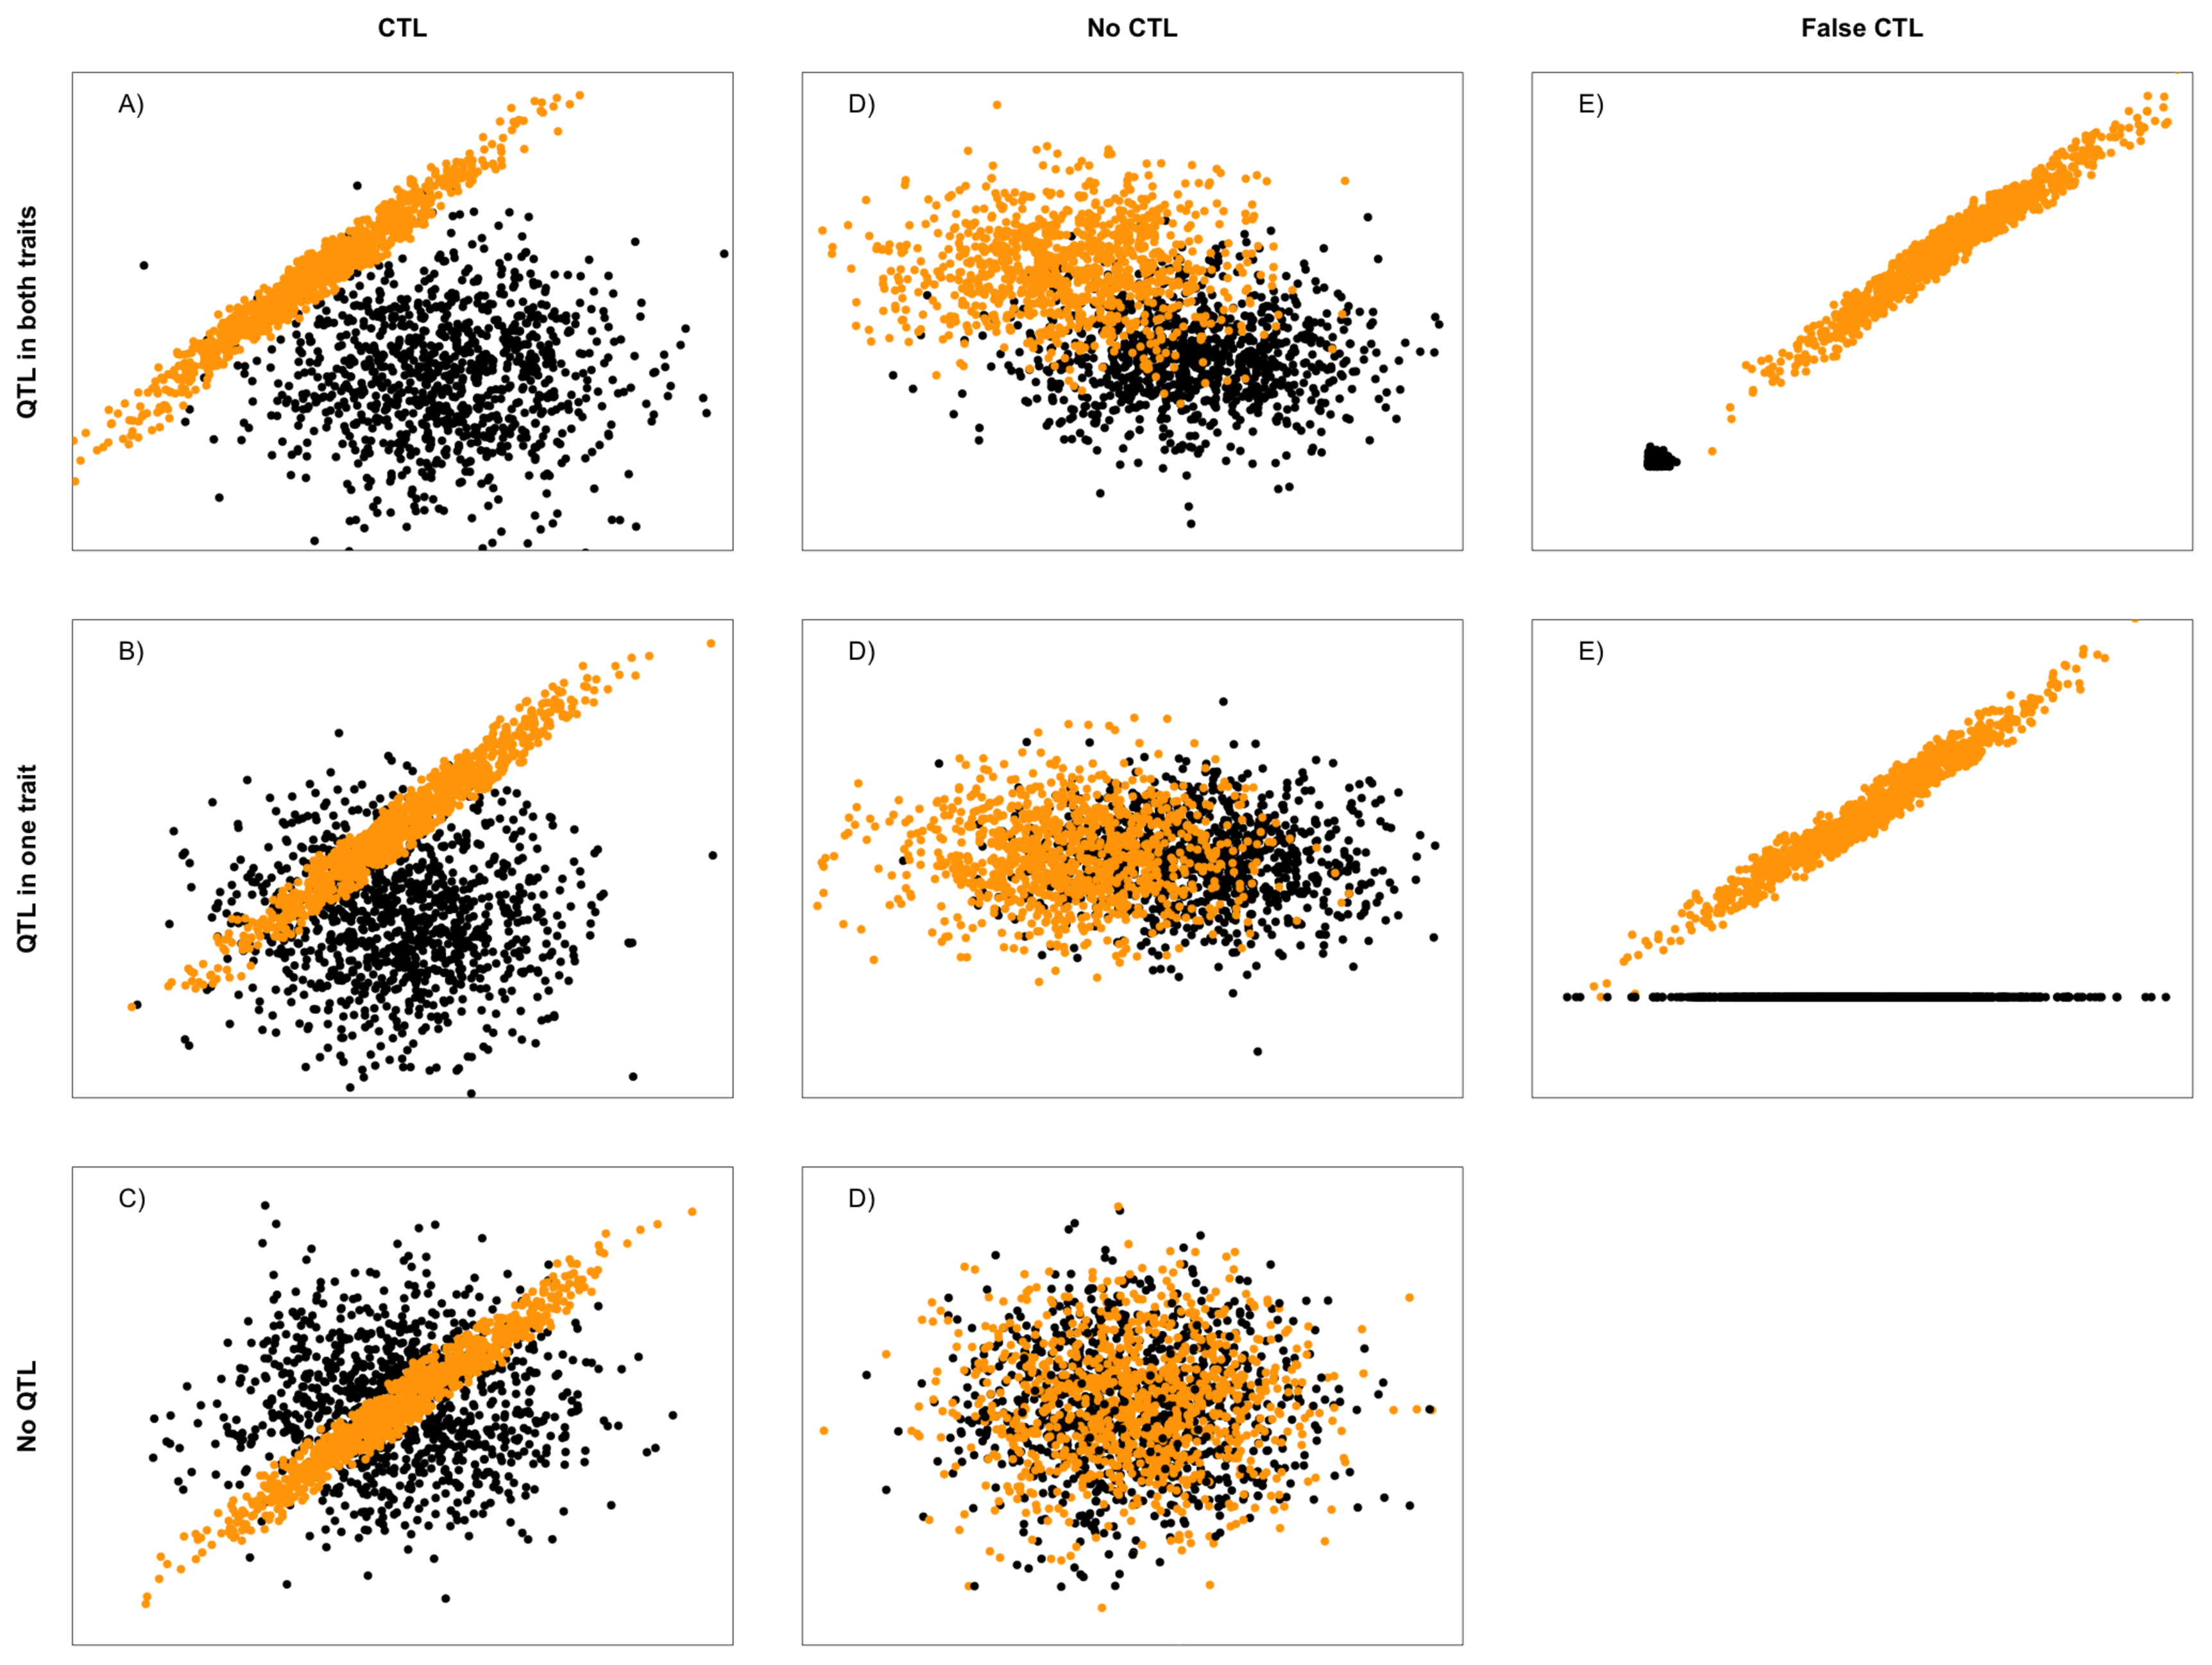
\includegraphics[width=0.9\textwidth]{eps/image_5_1.eps}
  \caption[CTLs.]{QTL and CTL analysis of two traits: a schematic of possible scenarios at a given marker. A trait can 
          have a QTL or no QTL at the given marker: there are four possible combinations in QTL analysis with two traits. 
          The trait pair can also have a CTL or no CTL and in the combined QTL and CTL analysis: the total number of possible 
          combinations is eight. Three additional scenarios refer to special cases when one trait or both traits are not 
          expressed in one genotype. For sake of simplicity it is assumed in this figure that there are two genotypes only, 
          e.g. as in a BC or RIL population. [We also ignore possible info on cis- and trans-mapping for the moment]}
          \label{fig:ctls}
  \end{figure}

  \subsection{QTL and CTL analysis of two traits}
  
  To describe the possible relationships between QTL and CTL we generate the possible scenario's as in figure \ref{fig:ctls}.\\
  {\bf(A)} The two traits have a QTL and a CTL at the given marker (1 scenario). This example shows the extreme scenario when the traits are 
  well correlated in one genotype and entirely uncorrelated in the other. The locus affects both the mean and the correlation. They could 
  have a regulatory factor in common, the effect of which is detected in QTL and CTL analysis.\\
  {\bf(B)} The two traits have a CTL at the given marker, but only one trait has a QTL at that marker (2 scenarios).  The locus affects the 
  correlation, and the mean of one trait only. They could have a regulator in common in which case the latter trait is downstream of the other 
  trait: this can happen e.g. if the locus leads to functionally different transcripts at equal expression levels for the trait without QTL, 
  and this effect is propagated to the trait with (therefore) a QTL.\\
  {\bf(C)} The two traits have a CTL but no QTL at the given marker (1 scenario). This example shows the extreme scenario when the traits 
  are well correlated in one genotype and entirely uncorrelated in the other.  The locus affects the correlation only. They could have a 
  regulatory factor in common, the effect of which is detected in CTL analysis only: e.g. if the locus leads to co-regulated transcription 
  in one genotype only.\\
  {\bf(D)} The two traits have no CTL at the given marker  (4 scenarios).  The locus does not change the correlation, it change the mean 
  if one or both traits have a QTL. The example shows the extreme scenario when both traits have a QTL but are entirely uncorrelated: they 
  could be downstream of the same or a different factor at the given region.\\
  {\bf(E)} The two traits have a CTL at the given marker, but the trait values are at the noise level in one genotype for one or both 
  traits (3 scenarios). This expression at noise level for one trait could result from e.g. hybridization failure for one genotype. One 
  or both traits can have a possibly artificial QTL and the two traits have a possibly artificial CTL. The example shows the scenario 
  when only one trait has a QTL.

\section{Inference of hierarchical relationship between traits}
  \subsection{Using information of co-localized CTL and QTL}
  Observing a significant CTL between T1 and T2 means that there is a factor (e.g. genetic regulator) located underneath 
  the CTL peak influencing the correlation between T1 and T2. This information of shared genetic control, therefore, 
  indicates that T1 and T2 are involved in the same biological pathway \cite{Tesson:2010}.

  The absence of QTL in trait T1 and the presence of QTL in trait T2 indicate that T2 is downstream of T1 in the 
  hierarchical network. The reasoning is that the variation caused by a genetic factor in T2 (QTL) has not 
  propagated to T1 \cite{Jansen:2009}. The reserve situation can also happen: Presence of QTL in trait T1 and the 
  absence of QTL in trait T2 indicate that T2 is upstream of T1 in the hierarchical network.

  The presence of QTL in both traits X and Y further confirms that T1 and T2 are related in the same pathway, and it 
  even allows us to go from inferring hierarchical relationship to causality using methods such as conditional 
  correlation \cite{Schadt:2007, Li:2010}.

  It should be noted that the co-localized CTL information does not exclude the existence of intermediate factor(s) 
  e.g. Z,  between T1 and T2 in the pathway, although the relative strength of correlation provides us 
  information on the distance among them in the network, e.g. higher correlation can indicate a shorter distance 
  between T1 and T2 in the network.\\

  \subsection{Using information of co-localized CTLs}
  When the CTLxy of X and Y co-localizes with CTLxz of X and Z and CTLyz of Y and Z, these three traits are possibly 
  involved in the same network. The relative effect sizes of these CTLs can be used to infer the order of X, Y and Z
  in the hierarchical network. For example, when CTLxy and CTLyz are larger than CTLxz, we can conclude that they 
  follow the order of X-Y-Z in the network, i.e. Y is in between of X and Z.

  Additionally when a QTL shows two or more co-localizing CTL we discovered a set of possible downstream targets 
  for the QTL. Which, when sample sizes permit, can be further annotated using gene ontology \cite{GeneOntology:2000} or 
  untangled by using methods like hierarchical inference (this paper) or causal inference \cite{Schadt:2005, Li:2006} 
  to obtain en even more detailed view of genetic regulation within the set.

  \subsection{Visualizing CTL information}
  Information obtained by CTL mapping can be visualized in several different ways the author found the most accessible 
  representation is a user-customizable network view. User customization helps researchers to add their own and/or 
  literature information to a network allowing for a rich interpretation of the created network. Network generated from 
  CTL mapping can be visualized by software tools including Cytoscape \cite{Cytoscape:2010, Cytoscape:2003}.

  CTL information allows us to draw lines from traits via markers to other traits reconstructing the underlying genetic 
  wiring. To create hierarchical networks we transforming the significant CTLs into network edges. This is done by 
  using a user defined genome wide FDR and then only transforming significant trait-marker-trait interactions into a 
  .sif network file.

\section{Cell type specific eQTL mapping in human GAWA data}
\label{sec:cellspecificeqtl}
  The number of available expression quantitative trait locus (eQTL) datasets from individual cell 
  types is limited because purifying cell types from mixtures is often challenging.  Since whole 
  peripheral blood is easily accessible and comprises many different cell-types, we developed 
  methodology to infer the specific cell-types in which eQTLs are operating,  alleviating the need 
  to sort cells and enabling interrogation of cell-types that are difficult to purify.

  We investigated whole peripheral blood of 5,683 unrelated individuals, and found that at least 
  8.5\% of all blood \emph{cis}-eQTLs are mediated by specific immune cell-types. Additionally, to our 
  knowledge, we present the first eQTL results for neutrophil granulocytes, a cell type that is 
  difficult to purify in the laboratory. We validated our findings in eQTL data of six purified 
  cell-types (lymphoblastoid cell-lines, B-cells, monocytes, CD4+ T-cells, CD8+ T-cells and 
  neutrophil granulocytes). Subsequent enrichment analysis of known disease-associated SNPs 
  revealed that Crohn's disease SNPs preferentially affect gene expression levels within neutrophil 
  granulocytes, underscoring the importance of neutrophils in Crohn's disease pathogenesis.

  \subsection{Background}
  In the past seven years, genome-wide association studies (GWAS) have identified thousands of genetic 
  variants that are associated with human disease\cite{Hindorff:2009}. The realization that many of 
  the disease-predisposing variants are noncoding, and that single nucleotide polymorphisms (SNPs) 
  often affect the expression of nearby genes (i.e. \emph{cis}-eQTLs) \cite{Powell:2012, Lude:2011, Zeller:2010}, 
  suggests these variants predominantly have a regulatory function. As such it is important to understand 
  in which specific tissues and cell-types these disease-associated variants exert their effect on disease.

  We have previously shown that whole peripheral blood is a suitable tissue to detect \emph{cis}-eQTL effects, 
  especially for SNPs that are associated with (auto) immune disorders \cite{Lude:2011, Westra:2013}. However, recent studies 
  suggest that disease-predisposing variants often exert their regulatory effect in a cell-type dependent 
  manner \cite{Brown:2013, Fairfax:2012, Fu:2012, Dimas:2009, Breitling:2008a}. This is problematic 
  when studying whole peripheral blood, since it is comprised out of   many different cell types that originate 
  from either the myeloid (e.g. neutrophil, granulocytes, monocytes) or lymphoid lineage (e.g. 
  B-cells or T-cells). An increase in the percentage of cells within one lineage decreases the 
  percentage of cells in the other (e.g. neutrophil percentage is strongly negatively correlated with 
  lymphocyte percentage; Supplementary Figure 1). Consequently, \emph{cis}-eQTLs that have been 
  detected in whole blood may actually reflect an effect within one single 
  cell-type, complicating the functional interpretation of disease predisposing variants. Although 
  several eQTL datasets have recently been presented on individual white blood cell types (for example, 
  monocytes\cite{Zeller:2010, Fairfax:2012} and T-cells \cite{Fairfax:2012, Ding:2010}), other white 
  blood cell types (particularly neutrophil granulocytes) are difficult to purify and culture in the lab 
  \cite{Grisham:1985}, even though they can reflect a substantial 
  proportion of circulating white blood cells (e.g. neutrophil granulocytes comprise approximately 62\% 
  of all peripheral blood mononuclear cells). In case eQTL datasets already exist for these individual 
  cell types, their sample-size is typically small, limiting statistical power to study the cell type 
  mediation of \emph{cis}-eQTLs in these cell types directly. As such, to our knowledge, we here present the 
  first eQTL analysis investigating neutrophil granulocytes.

  In this paper, we present a method that uses whole peripheral blood to infer in which cell-types these 
  eQTLs manifest themselves. We first estimate for each sample what the specific cell-type proportions 
  are (relying upon individual expression measurements of genes that serve as proxies for these cell-types) 
  and subsequently use a gene x environment interaction (G x E) model. This allows us to predict which 
  \emph{cis}-eQTLs are predominantly mediated by specific cell types in peripheral blood datasets that lack 
  any actual cell-count measurements. We apply our method to an unprecedented number of samples (5,683 
  unrelated whole peripheral blood samples from seven cohorts: EGCUT \cite{Metspalu:2004}, InCHIANTI 
  \cite{Tanaka:2009}, Rotterdam Study \cite{Hofman:2011}, Fehrmann \cite{Lude:2011}, SHIP-TREND 
  \cite{Teumer:2011}, KORA F4 \cite{Powell:2012, Mehta:2013}, and DILGOM \cite{Inouye:2010}). We 
  subsequently validate our predicted cell-type mediated eQTLs in six datasets of purified cell-types, and 
  observe that SNPs, associated with Crohn's disease are enriched for affecting gene expression levels in 
  neutrophil granulocytes.

  \subsection{Results}
  Identification of cell-type specific eQTLs in mixtures (e.g. whole peripheral blood) is most easily 
  understood when assuming an extreme situation where in half of all blood samples the proportion of 
  e.g. neutrophil granulocytes is very low, and in the other half of all blood samples this proportion 
  is actually high. If an eQTL of interest is not showing any effect in the samples with a very low 
  neutrophil granulocyte proportion, while showing a strong effect in the samples with a high proportion, 
  this suggests the eQTL is specific for neutrophil granulocytes. In order to apply this reasoning on 
  a whole blood dataset, the neutrophil percentage of each sample should be known and is used as a 
  covariate in a linear model that includes an interaction term (cell type percentage x genotype). 
  We applied this strategy to 5,683 samples and determined which of the 13,124 \emph{cis}-eQTLs that we have 
  discovered before5 are mediated by individual cell-types. We concentrated on neutrophil granulocytes, 
  since 1) they are the most abundant immune cell type in whole blood, 2) to our knowledge no previous 
  eQTL studies in neutrophil granulocytes have been published before and 3) a strong inverse 
  relationship exists between the neutrophil granulocyte percentage and the lymphocyte percentage in 
  blood (Supplementary Figure 1): as such if one is studying neutrophil percentage, one automatically 
  investigates lymphocyte percentage as well.

  However, neutrophil cell-count percentages were only available for the EGCUT and SHIP-TREND datasets. 
  To that end, we first developed a method that enabled us to approximate the cell type percentages for 
  datasets without cell type information (Figure 1). We used the EGCUT cohort to identify a list of 58 
  Illumina HT12v3 probes that strongly positively correlated (Spearman's correlation coefficient > 0.55) 
  with neutrophil granulocyte counts. We then summarized the information of these 58 individual probes 
  into a single neutrophil granulocyte count estimate, by applying principal component analysis (PCA) 
  and using the first principal component. We validated the accuracy of this 58 probe neutrophil count 
  predictor, by applying this procedure to the SHIP-TREND cohort and correlating the estimated neutrophil 
  percentage to the actual neutrophil percentage. We observed a strong correlation (Spearman's correlation 
  coefficient = 0.82; Supplementary Figure 2), indicating that these 58 probes jointly form a reliable 
  proxy for neutrophil percentage, and thus concluded we could use this procedure in the other cohorts 
  as well.

  Every cohort determined the interaction model for 13,124 \emph{cis}-eQTLs, while using the neutrophil 
  percentage proxy x genotype as interaction term. We subsequently meta-analyzed the interaction 
  terms for each \emph{cis}-eQTL (up to 5,683 samples were tested per eQTL) and identified 1,117 \emph{cis}-eQTLs 
  with a significant interaction effect (8.5\% of all tested cis-eQTLs; FDR < 0.05; 1,037 unique SNPs 
  and 836 unique probes; Table 1, Supplementary Table 1). 909 (6.9\%) had a positive direction of 
  effect, which indicates that these \emph{cis}-eQTLs show stronger effect sizes in neutrophil granulocytes 
  (302 eQTLs, 283 unique SNPs and 244 unique probes after a more stringent Bonferroni correction). We 
  will refer to these as neutrophil mediated \emph{cis}-eQTLs. Another 208 (1.6\%) had a negative direction of 
  effect (20 eQTLs, 20 unique SNPs and 13 unique probes after a more stringent Bonferroni correction), 
  indicating a stronger \emph{cis}-eQTL effect size in lymphoid cells (since lymphocyte percentages are 
  negatively correlated with neutrophil percentages, Supplementary Figure 1). We will refer to these 
  as lymphocyte mediated \emph{cis}-eQTLs. Overall, the directions of the significant interaction effects were 
  consistent across the different cohorts, indicating that our findings are robust (Supplementary 
  Figure 3). We did however observe that a large sample-size is essential in order to find these 
  cell-type mediated \emph{cis}-eQTLs (Figure 2): when studying fewer samples (ascertained by systematically 
  excluding more cohorts from our study) the number of significant cell-type mediated eQTLs decreases 
  quickly. This was particularly important for the lymphoid mediated \emph{cis}-eQTLs, since in blood, 
  myeloid cells are approximately twice as abundant as lymphoid cells, and consequently detection of 
  lymphoid mediated \emph{cis}-eQTLs is more challenging than detection of myeloid mediated \emph{cis}-eQTLs.

  We validated our findings in four purified cell-type gene expression datasets from the lymphoid 
  lineage (lymphoblastoid cell lines (LCLs), CD4+ T-Cells, CD8+ T-Cells and B-Cells; Figure 3, 
  Supplementary Table 2) and two purified cell-type datasets from the myeloid lineage (monocytes and 
  neutrophil granulocytes). As expected, compared to \emph{cis}-eQTLs without a significant interaction term 
  (generic \emph{cis}-eQTLs) the 909 neutrophil mediated \emph{cis}-eQTLs and the 208 lymphoid mediated \emph{cis}-eQTLs 
  indeed showed very strong \emph{cis}-eQTL effects in the myeloid datasets (Wilcoxon P-value < 4.9 x 10-31) 
  and lymphoid datasets (Wilcoxon P-value < 7.8 x 10-14), respectively (Figure 3). These results 
  indicate that our method is able to reliably predict whether a \emph{cis}-eQTL is mediated by a specific 
  cell type. We also assessed whether average gene expression levels within different cell-types might 
  be useful to predict whether a \emph{cis}-eQTL is mediated by a specific cell type, as it can be hypothesized 
  that if a certain gene is highly expressed within one single cell-type while it is only weakly 
  expressed in other cell-types, that the eQTL effect might manifest itself only in the highly expressed 
  cell-type. We indeed observed that, on average, the 909 neutrophil mediated and 208 lymphoid eQTL 
  genes showed slightly higher gene expression levels within the myeloid and lymphoid cell-types, 
  respectively (Supplementary Figure 3). However, for many individual genes that showed a strong 
  cell-type mediated \emph{cis}-eQTL effect, the average expression levels within that cell-type were not 
  higher than the other blood cell-types. As such, it is not possible to predict whether an eQTL is 
  operating in a particular cell-type by solely assessing in which cell-type the gene expression level 
  of this eQTL gene is the highest. 

  We next assessed whether there are immune related diseases, for which the associated SNPs 
  preferentially have affect gene expression within neutrophils (i.e. are enriched for neutrophil 
  mediated \emph{cis}-eQTLs).  We concentrated on 2 immune related diseases for which at least 30 unique 
  genome-wide significant (P < 5 x 10-8) loci have been identified before (as reported in the Catalog 
  of Published Genome-Wide Association Studies19, accessed September 23, 2013). Per disease, we tested 
  whether the associated SNPs were enriched for neutrophil mediated \emph{cis}-eQTLs by using a binomial test. 
  To ensure we tested independent loci, we first pruned the SNPs for linkage disequilibrium (R2 > 0.2). 
  We observed significant enrichment (one-tailed P = 0.001, Table 2) for Crohn's disease. Out of 51 
  unique SNPs that showed a \emph{cis}-eQTL effect, 11 were neutrophil mediated. These 11 SNPs affect the 
  expression of 14 unique genes (ZGPAT, LIME1, SLC2A4RG, CISD1, IL18RAP, HOTAIRM1, NOD2, AC034220.3, 
  SLC22A4, PLCL1, CPEB4, LGALS9, RP11-514O12.4, RNASET2).

  \subsection{Discussion}
  Here we have shown that it is possible to infer in which cell-types \emph{cis}-eQTLs are operating, without 
  the actual need to sort cells. We used whole peripheral blood eQTL data of 5,683 unrelated samples. 
  By first estimating cell-type proportions and subsequent use of a G x E (i.e. the estimated cell-type 
  proportions) interaction model we were able to demonstrate that hundreds of \emph{cis}-eQTLs show stronger 
  effects in myeloid than lymphoid cell-types and vice versa. 

  Since we could subsequently replicate these results in 6 individual purified cell-type eQTL datasets 
  (two reflecting the myeloid and four reflecting the lymphoid lineage), this indicates G x E analyses 
  can provide important additional biological insights for many SNPs that have previously been found 
  to be associated with complex (molecular) traits. 

  However, two main criteria apply in order to identify such G x E effects: first, sample size should 
  be large. Although, to our knowledge, this is the largest eQTL study that has been conducted so-far 
  (5,683 samples), it is clear by sampling subsets of the participating cohorts (Figure 2), that more 
  G x E effects should be detectable with even larger sample sizes. Secondly, choosing the appropriate 
  environmental factor is essential in order to find convincing G x E effects: although we found 1,117 
  \emph{cis}-eQTLs that were mediated by myeloid or lymphoid cell-types, a recent G x E study that aimed to 
  detect \emph{cis}-eQTLs that were mediated by either gender or age (assessed in 5,254 samples) found only 
  five G x E effects that replicated in an independent cohort20. As such the choice of environmental 
  factor is crucial in order to find G x E interaction effects.

  Here, we have concentrated on identifying \emph{cis}-eQTLs that are preferentially operating in either 
  myeloid or lymphoid cell-types. We did not attempt to assess this for specialized cell-types within 
  the myeloid or lymphoid lineage. However, this is well possible if cell-counts are available for 
  these cell-types, or if these cell-counts can be estimated by using the expression levels of genes 
  that serve as proxies for those cell-counts. As such, identification of cell-type mediated eQTLs 
  for previously unstudied cell-types is possible, without the actual need to generate any new data. 
  However, it should be noted that these individual cell-types typically have a rather low abundance 
  within whole blood (e.g. natural killer cells only comprise ~2\% of all circulating white blood 
  cells). As a consequence, in order to have sufficient statistical power to identify eQTLs that are 
  mediated by these cell-types, very large whole blood eQTL sample-sizes are required (analogous to 
  the substantially lower number of identified lymphoid mediated \emph{cis}-eQTLs, as compared to the myeloid 
  mediated \emph{cis}-eQTLs, since neutrophils are twice as abundant as lymphoid cells in whole blood). 
  Additionally, such cell-types should show differences in abundance across different individuals, 
  rendering identification of \emph{cis}-eQTLs that are specific for certain cell-types impossible if those 
  cell-types have a near equal abundance in blood across each of the individuals.

  In order to improve statistical power to detect cell-type mediated eQTLs, we corrected the gene 
  expression for technical and batch effects (here we applied principal component analysis and removed 
  per cohort the 40 strongest principal components that affect gene expression). Such procedures are 
  commonly used when conducting \emph{cis}-eQTL mapping \cite{Lude:2011, Dubois:2010, Fu:2012, Zhernakova:2013, Westra:2013, Lappalainen:2013}. Although this correction might diminish the 
  power to detect trans-eQTLs \cite{Westra:2013}, this concern does not apply to our G x E \emph{cis}-eQTL study: we first 
  determined the environment effect (i.e. neutrophil count percentage) for each individual samples by 
  combining the expression levels of 58 probes, based on the original expression data that was not 
  corrected for principal components. The subsequent G x E eQTL mapping was conducted on the expression 
  data that was corrected for principal components. Although for a specific G x E effect (e.g. a SNP 
  on chr. 6 in conjunction with neutrophil count percentage), the individual SNP or the individual 
  environmental factor might exert strong effects on overall blood gene expression levels (and thus 
  the SNP effect or the environmental factor effect might have been captured by any of the first 40 
  gene expression PCs), detection of the G x E effect will only become impossible when the specific 
  G x E effect (i.e. the specific combination of the SNP and environmental effect) would have been 
  captured by any of the first 40 gene expression PCs. We observed that the number of significantly 
  detected cell-type mediated \emph{cis}-eQTLs improved approximately two fold when correcting for these PCs, 
  without losing G x E effects that only had been detected in the uncorrected data (data not shown).

  We confined our analyses here to a subset of \emph{cis}-eQTLs for which we had previously identified a main 
  effect in whole peripheral blood \cite{Westra:2013}: for each \emph{cis}-eQTL gene, we here only studied the most 
  significantly associated SNP. Considering that for many \emph{cis}-eQTLs multiple, unlinked SNPs exist that 
  independently affect the gene expression levels, it is possible that we have missed myeloid or 
  lymphoid mediation of these secondary \emph{cis}-EQTLs.

  We anticipate that with the (pending) availability of large RNA-seq based eQTL datasets, statistical 
  power to identify cell-type mediated eQTLs will improve further: since RNA-seq enables very accurate 
  gene expression level quantitation and is not limited to a set of preselected probes that interrogate 
  well known genes (as is the case for microarrays), the detection of genes that can serve as reliable 
  proxies for individual cell-types will improve. Secondly, using RNA-seq data, it is possible to 
  assess whether SNPs that affect the expression of non-coding transcripts, affect splicing \cite{Lappalainen:2013} or result 
  in alternative polyadenylation \cite{Zhernakova:2013} are mediated by specific cell-types.

  Although we applied our method to whole blood gene expression data, our method can be applied to any 
  tissue, alleviating the need to sort cells or to perform laser capture micro dissection. The only 
  prerequisite is that eQTL data in such tissues is available for many samples. However, since an 
  increasing number of eQTL datasets in different tissues are now becoming available and eQTL meta-analyses 
  have proven successful \cite{Lude:2011, Westra:2013}, our approach provides a cost effective way to identify cell-type 
  mediated eQTLs, that is likely to reveal novel biological insight.

